% TPI Simulación 2026 - Régimen de campañas del horno de cementación (grupo Casermeiro)
% Formato paper (consigna del 28/10/2026): abstract, objetivos, metodología, resultados y conclusiones, con los
% diez pasos del estudio de simulación implícitos. Compila con pdfLaTeX + BibTeX (Overleaf) o con tectonic:
%   tectonic -X compile tpi-caser.tex
% Antes de entregar: grep 'pendiente{' para que no quede ninguna marca roja.
\documentclass[a4paper,11pt]{article}

\usepackage{iftex}
\ifPDFTeX
  \usepackage[T1]{fontenc}
  \usepackage[utf8]{inputenc}
  \usepackage{lmodern}
\else
  \usepackage{fontspec}  % tectonic / XeLaTeX: Latin Modern en Unicode
\fi
\usepackage[spanish,es-noshorthands,es-tabla]{babel}
\usepackage[margin=2.3cm]{geometry}
\usepackage{amsmath,amssymb}
\usepackage{booktabs,tabularx,array,makecell}
\usepackage{graphicx}
\usepackage{float}
\usepackage[font=small,labelfont=bf]{caption}
\usepackage{xcolor}
\usepackage{tikz}
\usetikzlibrary{arrows.meta,positioning,calc}
\usepackage[output-decimal-marker={,},group-separator={.},group-minimum-digits=4]{siunitx}
\usepackage{csquotes}
\usepackage[round,authoryear]{natbib}
\usepackage[hidelinks]{hyperref}

\setlength{\emergencystretch}{3em}
% figs/ dentro del zip de Overleaf; ../../../../figs/ al compilar desde el repo.
\graphicspath{{figs/}{../../../../figs/}}
\newcommand{\pendiente}[1]{\textcolor{red}{[PENDIENTE: #1]}}
\newcommand{\Md}{\,\mathrm{M\$}}

\title{\textbf{¿Cuándo encender el horno?}\\[0.3em]
\large Simulación de eventos discretos del régimen de campañas de un horno de cementación\\
en una PyME metalúrgica, con datos reales de operación, energía y gas}
\author{Augusto Brizio, Gonzalo Casermeiro, Jeremías Constantini,\\ Tiziano Messina y Juan Ignacio Navos\\[0.4em]
\small Universidad Tecnológica Nacional, Facultad Regional Rosario\\
\small Ingeniería en Sistemas de Información --- Simulación 2026\\[0.3em]
\small \pendiente{correos de los cinco autores}}
\date{Noviembre de 2026}

\begin{document}
\maketitle

\begin{abstract}
\noindent Una fábrica de tornillos opera un horno eléctrico de cementación y temple por campañas: lo enciende
cuando se acumulan unas 80 unidades de carga (ULI), lo calienta durante 36~h, procesa una ULI cada 85~min mientras
haya cola, lo mantiene caliente hasta 48~h por si llega más material y lo deja enfriar 48~h. Construimos en
AnyLogic un modelo de eventos discretos del horno, alimentado con un año de registros reales de lavado, la
distribución empírica del peso de las cargas y regresiones sobre las facturas de electricidad y de gas del
propio horno. El modelo reproduce cuatro de seis medidas históricas dentro de la tolerancia fijada de antemano. Comparamos la regla actual con tres
alternativas mediante 30 réplicas apareadas por escenario y números aleatorios comunes. Bajar el umbral de
encendido o fijar una espera máxima reduce la espera de las cargas, pero encarece la operación entre 2,9 y
4,8~M\$ por año. Apagar el horno apenas se vacía la cola, en cambio, reduce el costo relevante (luz, gas y capital
inmovilizado) en $18{,}0 \pm 1{,}8$~M\$ por año ($-21{,}5$\,\%), a cambio de 1,1 días más de espera media. El
resultado se mantiene en todo el rango de sensibilidad de los parámetros de costo.

\medskip\noindent\textbf{Abstract.} A small screw manufacturer runs its carburizing furnace in campaigns: it is
switched on after about 80 load units have accumulated, heated for 36~h, kept hot while there is work (and up to
48~h after the queue empties) and cooled for 48~h. We built a discrete-event model in AnyLogic fed with one year of
real shop-floor records and with regressions on the furnace's own electricity and gas bills. With 30 paired
replications per scenario and common random numbers, switching the furnace off as soon as the queue empties
lowers the yearly relevant cost by 21.5\,\% at the price of 1.1 extra days of average waiting time, while
lowering the start-up threshold or capping the waiting time increases it.

\medskip\noindent\textbf{Palabras clave:} simulación de eventos discretos, política de encendido por umbral,
política N, horno de tratamiento térmico, AnyLogic, números aleatorios comunes.
\end{abstract}

% ======================================================================================================
\section{Introducción}

La empresa estudiada, a la que llamamos \emph{Caser}, es una PyME metalúrgica de la provincia de Santa Fe que
fabrica tornillos autoperforantes, para techo y para muebles. El proceso es casi todo interno: estampado de la
cabeza, laminado de la rosca, lavado, tratamiento térmico (cementación y temple), cincado tercerizado y envasado.
El tratamiento térmico se hace en un horno eléctrico de cinta continua, de 27 resistencias, con un generador de
gas endotérmico a propano (GLP) que produce la atmósfera de cementación.

El horno trata las cargas \emph{de a una}: cada unidad de transporte interno (ULI, un contenedor de unos 140~kg de
piezas) recorre la cinta en media hora y entra una cada 85~min, en tres turnos de 8~h. Lo que lo convierte en un
sistema por lotes no es su capacidad sino su costo de arranque: necesita 36~h de calentamiento antes de la
primera carga y 48~h de enfriamiento después de la última, y durante todo el tiempo que está a temperatura
consume electricidad y gas aunque no tenga nada que tratar. Con la planta subutilizada, el horno pasa la mayor
parte del tiempo apagado y se enciende por campañas.

La regla actual la aplica el encargado de planta sin un procedimiento escrito: enciende cuando se juntan entre
70 y 80 ULI lavadas (o antes, si hay un pedido urgente), carga mientras haya cola y, cuando la cola se vacía,
mantiene el horno caliente hasta dos días por si llega más material. La empresa nos planteó la pregunta
concreta de \emph{cuántas ULI conviene esperar antes de encender}. Esperar más reparte el costo de arranque entre
más kilos, pero alarga la espera del material, inmoviliza capital y demora las entregas. Es la disyuntiva clásica
de las colas con servidor removible y política de encendido por umbral, o política $N$
\citep{yadin1963,heyman1968}. En este caso, sin embargo, el arranque dura días, los arribos no son Poisson y los
costos salen de facturas reales, lo que obliga a simular en lugar de usar las fórmulas cerradas de esos modelos.

% ======================================================================================================
\section{Objetivos}

\textbf{Objetivo general.} Evaluar con un modelo de simulación validado si alguna regla de encendido y apagado
del horno reduce el costo relevante de operarlo sin deteriorar de forma inaceptable la espera del material, y
emitir una recomendación fundada en evidencia estadística.

\textbf{Objetivos específicos.}
\begin{enumerate}
  \item Representar el horno como un servidor con preparación larga y encendido por umbral, con las cargas como
        agentes individuales, para medir la espera de cada ULI y el tiempo del horno en cada estado.
  \item Construir las entradas del modelo con datos reales de la empresa: arribos de ULI lavadas, peso por
        ULI, consumo de electricidad y de GLP, tarifas y costo del capital.
  \item Verificar el programa contra un caso con solución analítica y validarlo contra el registro histórico
        del mismo período que las entradas.
  \item Comparar la regla actual con tres alternativas (umbral más bajo, espera máxima y apagado inmediato)
        mediante corridas múltiples y un test de medias apareado.
  \item Cuantificar la robustez de la conclusión frente a los parámetros de costo más inciertos.
\end{enumerate}

% ======================================================================================================
\section{Metodología}

\subsection{Sistema y modelo conceptual}

El estudio abarca el horno y su cola de entrada. Lo que ocurre antes del lavado se resume en el proceso de
arribos de ULI lavadas, y lo que ocurre después del horno queda fuera del sistema. La entidad es la ULI, con sus
atributos de peso, instante de llegada y urgencia; la campaña no es una entidad sino un estado del horno. La
unidad de tiempo es la hora, y el modelo arranca un lunes a las 00:00 con la cola vacía y el horno apagado.

El horno tiene cinco estados (figura~\ref{fig:estados}). Pasa de \emph{Apagado} a \emph{Acumulando} con la
primera ULI en cola, y de \emph{Acumulando} a \emph{Calentando} cuando ocurre lo primero de tres eventos: que la
cola alcance el umbral, que llegue una ULI urgente, o que la ULI más vieja cumpla la espera máxima (si la regla la
define). Tras 36~h pasa a \emph{Procesando}, donde carga una ULI cada 85~min, urgentes primero y después en orden
de llegada. Si la cola se vacía, el horno queda caliente y en vacío: una llegada reanuda la carga, y si no llega
nada en el tiempo de espera en vacío, pasa a \emph{Enfriando} y, 48~h después, a \emph{Apagado}. Un encendido por
urgencia trata la cola que haya y enfría sin esperar.

\begin{figure}[H]
\centering
\begin{tikzpicture}[
  st/.style={draw, rounded corners=6pt, minimum width=2.3cm, minimum height=0.9cm, align=center, font=\small, fill=#1},
  st/.default={gray!8},
  tr/.style={-{Stealth[length=2.2mm]}, thick},
  lb/.style={font=\scriptsize, align=center}]
  \node[st] (ap) {Apagado};
  \node[st, right=1.8cm of ap] (ac) {Acumulando};
  \node[st=orange!15, right=2.6cm of ac] (ca) {Calentando\\36 h};
  \node[st=blue!12, below=1.6cm of ca] (pr) {Procesando\\85 min/ULI};
  \node[st=cyan!10, left=2.6cm of pr] (en) {Enfriando\\48 h};
  \draw[tr] (ap) -- node[above, lb] {llega\\una ULI} (ac);
  \draw[tr] (ac) -- node[above, lb] {cola $\geq$ umbral, o urgente,\\o espera máxima} (ca);
  \draw[tr] (ca) -- node[right, lb] {fin del\\calentamiento} (pr);
  \draw[tr] (pr) -- node[above, lb] {cola vacía durante\\la espera en vacío} (en);
  \draw[tr] (en) -| node[pos=0.25, below, lb] {fin del enfriamiento} (ap);
  \draw[tr] (pr.east) to[out=20, in=-20, looseness=5] node[right, lb] {carga mientras\\haya cola} (pr.east);
\end{tikzpicture}
\caption{Estados del horno. La espera en vacío vale 48~h en la regla actual y 0~h en el escenario E3.}
\label{fig:estados}
\end{figure}

El modelo conceptual (estados, regla de encendido, carga mientras haya cola, prioridad de las urgentes) se
revisó con el encargado del horno antes de programarlo y se corrigió con sus respuestas. Una de esas
correcciones fue decisiva: en una primera entrevista se había anotado que las ULI que llegan con el horno
encendido esperan la campaña siguiente, pero el registro lo contradecía y el encargado confirmó que se cargan
igual. También confirmó que los encendidos anticipados por urgencia tratan toda la cola presente.

\subsection{Datos de entrada}

Todas las entradas salen de registros de la empresa (tabla~\ref{tab:entradas}). El seguimiento de ULI del
sistema de gestión registra, para 11.353 cargas de 2024 a 2026, las fechas de lavado y de cementado y el
peso. Los arribos se modelan con los últimos 12 meses (18/08/2025 al 14/08/2026), para no mezclar niveles de
actividad distintos.

\textbf{Arribos.} La cantidad diaria de ULI lavadas no se ajusta a ninguna distribución teórica: el 49\,\% de
los días hábiles no hay lavado, hay picos de 10 a 20 ULI y los días de una misma semana están correlacionados
(autocorrelación de 0,43), porque el lavado sigue a órdenes de fabricación que duran varios días. Por eso se
usa un \emph{bootstrap} por semanas completas: cada lunes el modelo sortea una de las 52 semanas reales y
reproduce sus cinco días hábiles, con la hora de llegada uniforme entre las 6 y las 22. Así se conservan la
proporción de días vacíos, los picos y la correlación dentro de la semana, con una media de 33,6~ULI por semana.

\textbf{Peso por ULI.} Distribución empírica (101 cuantiles, media 140,9~kg, mediana 131,6~kg) muestreada por
transformada inversa.

\textbf{Energía y gas.} El medidor eléctrico del horno fue exclusivo hasta abril de 2026, lo que permite una
regresión mensual de las facturas sobre la cantidad de encendidos y los días a temperatura:
$\text{kWh}_{\text{mes}} = a + b \cdot \text{encendidos} + c \cdot \text{días calientes}$, con
$b = 2.303$~kWh por encendido (que incluye el calentamiento), $c = 2.402$~kWh por día caliente y $R^2 = 0{,}90$.
El costo marginal de la energía (102~\$/kWh) es la pendiente del importe contra los kWh facturados ($R^2 =
0{,}95$): el cargo fijo de potencia no depende de la regla de encendido y no se imputa. El GLP del generador
endotérmico sale de las facturas del proveedor completadas con la estadística de compras de la empresa
(enero de 2024 a agosto de 2026): unos 130~kg por día caliente ($R^2 = 0{,}92$), sin un término por encendido
significativo.

\textbf{Capital inmovilizado.} Se valoriza el material que espera en cola a 4.467~\$/kg (precio de lista por
el factor de costo de la empresa, ponderado por la mezcla de los últimos 12 meses), con la tasa del 2\,\%
mensual que usa la empresa. Es una cota superior, porque el material todavía no tiene el valor del producto
terminado.

\begin{table}[H]
\centering\small
\caption{Parámetros del modelo y su origen.}
\label{tab:entradas}
\begin{tabularx}{\textwidth}{@{}l r X@{}}
\toprule
Parámetro & Valor & Origen \\
\midrule
Umbral de encendido & 79 ULI & Cola media al encender en las campañas largas 2024-2026 (el encargado relevó 70-80) \\
Tiempo por ULI & 85 min & 17 ULI por día en tres turnos (encargado) \\
Calentamiento / enfriamiento & 36 h / 48 h & Relevado \\
Espera caliente en vacío & 48 h & Huecos de 1-2 días sin carga dentro de las campañas reales \\
Probabilidad de urgencia & 0,0054 & 10 encendidos anticipados / 1.857 ULI llegadas con el horno apagado \\
Electricidad & \makecell[r]{2.303 kWh/encendido\\2.402 kWh/día caliente} & Regresión de facturas del medidor exclusivo ($R^2 = 0{,}90$) \\
Tarifa marginal & 102 \$/kWh & Importe contra kWh, facturas 03/2025-04/2026 ($R^2 = 0{,}95$) \\
GLP & 130 kg/día caliente & Facturas y compras 2024-2026 ($R^2 = 0{,}92$); precio 2.250 \$/kg con impuestos \\
Valor del material / tasa & 4.467 \$/kg / 2\,\% mensual & Lista de precios y empresa \\
\bottomrule
\end{tabularx}
\end{table}

\subsection{Implementación en AnyLogic}

El modelo usa la Process Modeling Library de AnyLogic~8.9 \citep{borshchev2013,anylogic2026}: \texttt{Source}
$\rightarrow$ \texttt{Wait} (cola del horno) $\rightarrow$ \texttt{Delay} de capacidad~1 (el horno)
$\rightarrow$ \texttt{Sink}. La cola es un \texttt{Wait} y no un \texttt{Queue} porque el horno decide
\emph{cuál} ULI carga y \emph{si} carga: una función de despacho libera la ULI elegida solo en el estado
\emph{Procesando}. No se usa el bloque \texttt{Batch}, porque agrupar 80 ULI en un lote ocultaría justamente lo
que se quiere medir: la espera individual de cada carga y las ULI que se suman a una campaña ya encendida. La
lógica de estados vive en funciones y eventos del agente principal, y el statechart la refleja para la
animación.

Cada fuente de aleatoriedad (arribos, peso, urgencia, tiempo de ciclo) tiene su propio generador, sembrado a
partir de la semilla de la réplica. Como ninguno depende del estado del horno, con la misma semilla todos los
escenarios reciben exactamente las mismas ULI en los mismos instantes: es la condición para usar números
aleatorios comunes \citep[cap.~11]{law2015}. Cada corrida escribe una fila con 38 medidas en un CSV.

\subsection{Verificación}

El programa se verificó de tres formas. Primero, se extrajo el código del \texttt{.alp} y se compiló contra la
API instalada de AnyLogic. Segundo, se ejecutó en un motor de eventos discretos mínimo con trazas de resultado
conocido: umbral, calentamiento, carga en vacío cancelada por una llegada, enfriamiento, consumo, espera
máxima, prioridad, conservación de ULI (entradas = tratadas + en cola + en el horno) e invariancia ante el orden
de eventos simultáneos. Tercero, se corrió un caso degenerado con solución analítica: con umbral~1, sin
calentamiento, enfriamiento ni espera en vacío, arribos Poisson ($\lambda = 0{,}7$/h) y ciclo exponencial ($\mu
= 1$/h), el horno es una cola M/M/1 (tabla~\ref{tab:mm1}). Por último, las 120 corridas del experimento en
AnyLogic coincidieron campo por campo con las del motor mínimo.

\begin{table}[H]
\centering\small
\caption{Caso degenerado M/M/1: modelo contra teoría (12.000 días, 5 semillas).}
\label{tab:mm1}
\begin{tabular}{@{}lrrr@{}}
\toprule
Medida & Modelo & Teoría & Error \\
\midrule
$L_q$ (ULI en cola) & 1,6319 & 1,6333 & $-0{,}09$\,\% \\
$L$ (ULI en el sistema) & 2,3317 & 2,3333 & $-0{,}07$\,\% \\
$W$ (h en el sistema) & 3,3305 & 3,3333 & $-0{,}09$\,\% \\
$W_q$ (h en cola) & 2,3309 & 2,3333 & $-0{,}11$\,\% \\
$\rho$ (utilización) & 0,6998 & 0,7000 & $-0{,}02$\,\% \\
\bottomrule
\end{tabular}
\end{table}

\subsection{Validación}

El escenario base se comparó con el registro del mismo período que las entradas, con tolerancias fijadas antes
de correr: error relativo de la media de 10\,\% para las medidas de campaña y de 15\,\% para la espera y los kWh,
complementado con un intervalo de Welch para la diferencia entre las observaciones reales y las réplicas
\citep[cap.~5]{law2015}. Ninguna de estas medidas se usó para fijar parámetros: calibrar no es validar. La espera
se compara sin el 8\,\% de ULI que el registro muestra retenidas más de 30 días por falta de demanda, una
decisión comercial que el modelo no representa.

\begin{table}[H]
\centering\small
\caption{Validación del escenario base contra el registro (30 réplicas).}
\label{tab:validacion}
\begin{tabular}{@{}lrrrrl@{}}
\toprule
Medida & Registro & Modelo & Error & Tolerancia & Veredicto \\
\midrule
Toneladas tratadas por mes & 21,6 & 21,1 & $-2{,}5$\,\% & 10\,\% & dentro \\
Duración de la campaña (días) & 9,82 & 9,68 & $-1{,}4$\,\% & 10\,\% & dentro \\
Espera media sin retenidas (días) & 7,38 & 6,52 & $-11{,}7$\,\% & 15\,\% & dentro \\
kWh del horno por mes & 38.000 & 33.500 & $-11{,}8$\,\% & 15\,\% & dentro \\
Campañas por mes & 0,94 & 1,08 & $+15{,}3$\,\% & 10\,\% & fuera \\
ULI por campaña & 114 & 139 & $+21{,}9$\,\% & 10\,\% & fuera$^{a}$ \\
\bottomrule
\multicolumn{6}{@{}l}{\footnotesize $^{a}$ Con 11 campañas en el período, el intervalo de Welch contiene al cero: la diferencia no es significativa.}
\end{tabular}
\end{table}

El modelo mueve la cantidad correcta de material, con campañas de la duración correcta, y reproduce la espera
media y el consumo. Enciende algo más seguido que la realidad, lo que sesga a la baja la espera y al alza el
costo de arranque. Como esa medida se mueve en la misma dirección en todos los escenarios, afecta poco a
la comparación entre ellos, que es lo que el estudio usa.

\subsection{Diseño de experimentos}

\textbf{Escenarios.} Además de la regla actual se evalúan tres alternativas, todas con la misma prioridad para
urgentes (tabla~\ref{tab:escenarios}). E1 y E2 apuntan a reducir la espera. E3 responde a la práctica del
encargado de mantener el horno caliente cuando cree que llegará más material, y evalúa la alternativa opuesta.

\begin{table}[H]
\centering\small
\caption{Escenarios.}
\label{tab:escenarios}
\begin{tabular}{@{}llrrr@{}}
\toprule
& Descripción & Umbral (ULI) & Espera máxima & Espera en vacío \\
\midrule
E0 & Regla actual & 79 & --- & 48 h \\
E1 & Umbral bajo & 45 & --- & 48 h \\
E2 & Umbral con espera máxima & 79 & 15 días & 48 h \\
E3 & Apagar apenas se vacía la cola & 79 & --- & 0 h \\
\bottomrule
\end{tabular}
\end{table}

\textbf{Horizonte y calentamiento.} El sistema no tiene un instante natural de fin, por lo que se trata como no
terminante: cada réplica descarta un período de calentamiento y mide 365 días. El período se determinó con el
método gráfico de \citet{welch1983} sobre corridas piloto sin calentamiento \pendiente{resultado de Welch: corte y
justificación de los 90 días; figura tpi-caser-welch.png}.

\textbf{Réplicas y números aleatorios comunes.} Cada escenario se corre con 30 réplicas; la réplica $j$ usa la
semilla $j$ en los cuatro escenarios \pendiente{precisión relativa lograda con 30 réplicas}. En AnyLogic las
120 corridas se ejecutan con un experimento de variación de parámetros, con la semilla como parámetro y no
con la opción de replicaciones del experimento, que asigna semillas al azar.

\textbf{Test de medias.} Para cada alternativa $k$ y cada medida, se calculan las diferencias apareadas
$D_j = X_{k,j} - X_{0,j}$, $j = 1,\dots,n$, y el intervalo de confianza $t$ apareado \citep[cap.~10]{law2015}:
\begin{equation}
\bar{D} = \frac{1}{n}\sum_{j=1}^{n} D_j, \qquad
s_D^2 = \frac{1}{n-1}\sum_{j=1}^{n}\left(D_j - \bar{D}\right)^2, \qquad
\bar{D} \pm t_{n-1,\,1-\alpha/2}\,\frac{s_D}{\sqrt{n}} .
\end{equation}
Si el intervalo no contiene al cero, la diferencia es significativa y el intervalo indica su tamaño. Si lo
contiene, no hay evidencia de diferencia, y ese es un resultado válido. El apareamiento no exige
varianzas iguales ni independencia entre escenarios: aprovecha la correlación positiva que inducen los números
aleatorios comunes. Las tres medidas primarias (costo relevante del año, espera media y kilos en cola) se
evalúan con corrección de Bonferroni, $\alpha = 0{,}05/3$ por intervalo ($t_{29;\,0{,}9917} = 2{,}541$), para que
la conclusión conjunta mantenga una confianza del 95\,\%. Las secundarias se informan al 95\,\%
($t_{29;\,0{,}975} = 2{,}045$).

\textbf{Costo relevante.} Es la suma de lo que cambia con la regla de encendido: electricidad (consumo por
encendido y por hora caliente, a tarifa marginal), GLP por hora caliente y costo financiero del material en cola.

% ======================================================================================================
\section{Resultados}

La tabla~\ref{tab:resultados} resume las medias de las 30 réplicas de cada escenario. Los cuatro tratan la
misma cantidad de material (unas 252~t por año) y tienen la misma utilización del horno (29\,\%), porque reciben
las mismas ULI. Lo que cambia es cuánto tiempo pasa el horno caliente y cuánto espera el material.

\begin{table}[H]
\centering\small
\caption{Medias por escenario (30 réplicas, 365 días medidos). Costos en millones de pesos por año.}
\label{tab:resultados}
\begin{tabular}{@{}lrrrr@{}}
\toprule
Medida & E0 & E1 & E2 & E3 \\
\midrule
Costo relevante del año (M\$) & 83,7 & 88,5 & 86,5 & \textbf{65,7} \\
\quad Electricidad & 37,6 & 41,1 & 39,5 & 29,2 \\
\quad GLP & 41,3 & 44,5 & 43,0 & 30,9 \\
\quad Capital inmovilizado & 4,8 & 2,9 & 4,1 & 5,6 \\
Fracción del tiempo a temperatura & 38,7\,\% & 41,7\,\% & 40,3\,\% & 28,9\,\% \\
kWh por kg tratado & 1,46 & 1,60 & 1,54 & 1,14 \\
Encendidos por año & 12,9 & 16,2 & 14,7 & 14,2 \\
ULI por campaña & 139 & 111 & 123 & 127 \\
Espera media antes del horno (días) & 6,5 & \textbf{4,0} & 5,6 & 7,6 \\
Espera p90 (días) & 14,4 & 8,3 & 12,2 & 16,2 \\
Espera máxima (días) & 32,5 & 27,4 & 16,9 & 35,6 \\
Kilos promedio en cola & 4.437 & 2.700 & 3.815 & 5.200 \\
\bottomrule
\end{tabular}
\end{table}

La tabla~\ref{tab:test} presenta los intervalos apareados de las medidas primarias. Todas las diferencias
contra la regla actual son significativas.

\begin{table}[H]
\centering\small
\caption{Intervalos apareados de la diferencia contra E0 ($\bar{D} \pm$ semiamplitud), medidas primarias,
nivel individual 98,3\,\% (Bonferroni). Negativo: el escenario es menor que E0.}
\label{tab:test}
\begin{tabular}{@{}lrrr@{}}
\toprule
Medida & E1 $-$ E0 & E2 $-$ E0 & E3 $-$ E0 \\
\midrule
Costo relevante (M\$/año) & $+4{,}82 \pm 1{,}68$ & $+2{,}87 \pm 0{,}82$ & $-18{,}00 \pm 1{,}79$ \\
Espera media (días) & $-2{,}57 \pm 0{,}36$ & $-0{,}96 \pm 0{,}38$ & $+1{,}11 \pm 0{,}34$ \\
Kilos en cola & $-1.736 \pm 218$ & $-621 \pm 210$ & $+764 \pm 221$ \\
\bottomrule
\end{tabular}
\end{table}

\begin{figure}[H]
\centering
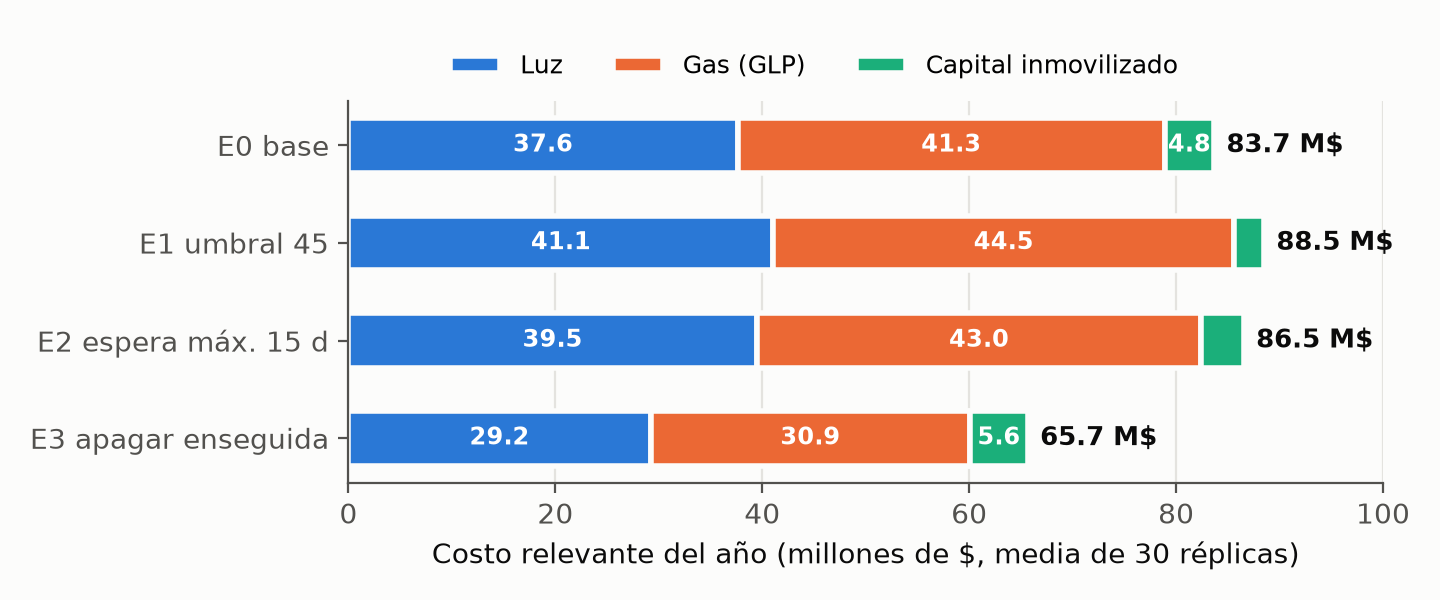
\includegraphics[width=0.92\textwidth]{tpi-caser-costos.png}
\caption{Composición del costo relevante del año por escenario.}
\label{fig:costos}
\end{figure}

\textbf{Bajar el umbral (E1) o fijar una espera máxima (E2)} reduce la espera, 2,6 y 1,0 días de media
respectivamente, y el material inmovilizado. Pero enciende más veces y mantiene el horno más tiempo
caliente con poca carga: el ahorro financiero (1,9~M\$ en E1) no compensa el aumento de energía (6,7~M\$). Con
la demanda actual, ninguna de las dos se justifica por costo. Solo convendría si la menor espera tuviera un
valor comercial (entregas más rápidas, ventas que hoy se pierden) mayor que esos 2,9 a 4,8~M\$ anuales.

\textbf{Apagar enseguida (E3)} ahorra $18{,}0 \pm 1{,}8$~M\$ por año, el 21,5\,\% del costo relevante. El
ahorro viene de eliminar el tiempo en que el horno está caliente y vacío: en E0 el horno está a temperatura el
38,7\,\% del año pero procesando solo el 29\,\%, de modo que una cuarta parte del tiempo caliente es espera en
vacío. E3 lleva la fracción caliente a la utilización, unas 850~h menos por año. A cambio, las ULI que llegan
después de un apagado esperan la campaña siguiente: la espera media sube 1,1 días, el p90 1,8 días y el horno
se enciende 1,3 veces más por año (figura~\ref{fig:compromiso}).

\begin{figure}[H]
\centering
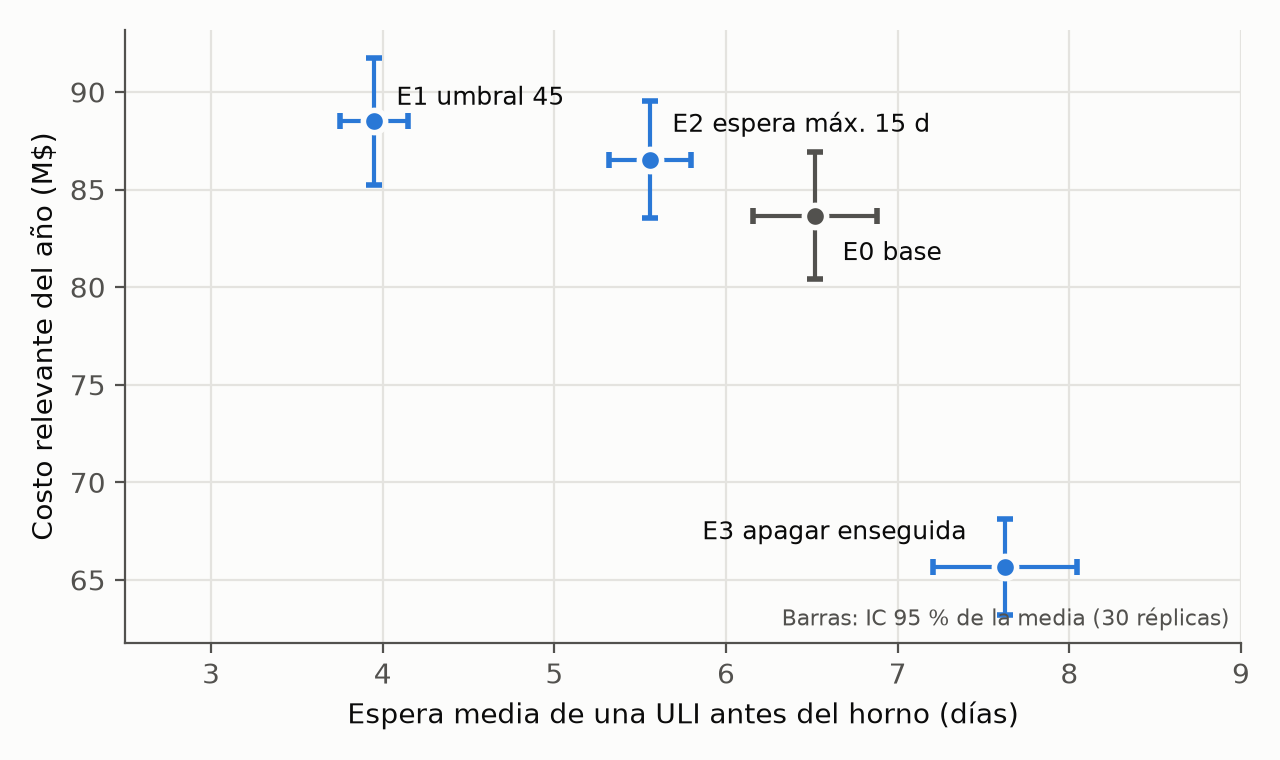
\includegraphics[width=0.78\textwidth]{tpi-caser-compromiso.png}
\caption{Costo contra espera por escenario. Las barras son intervalos de cada media; la comparación formal es
la de la tabla~\ref{tab:test}, apareada, con intervalos mucho más estrechos.}
\label{fig:compromiso}
\end{figure}

\textbf{Sensibilidad.} Los parámetros de costo no alteran la dinámica del modelo (cuándo se enciende el horno,
cuánto espera cada ULI): solo entran en el cálculo final. Por eso la sensibilidad a ellos se obtiene exacta
recalculando el costo sobre las mismas 120 corridas (tabla~\ref{tab:sensibilidad}). El ahorro de E3 se
mantiene en todos los casos. El supuesto que más lo amenaza es un costo por encendido que el modelo no incluye
(desgaste de resistencias, cinta y mufla): para anular el ahorro, ese costo tendría que llegar a 14,2~M\$ por
encendido, del orden de lo que cuesta un mes entero de operación.

\begin{table}[H]
\centering\small
\caption{Sensibilidad de la diferencia de costo relevante contra E0 (M\$/año, IC 98,3\,\%).}
\label{tab:sensibilidad}
\begin{tabular}{@{}lrrr@{}}
\toprule
Caso & E1 $-$ E0 & E2 $-$ E0 & E3 $-$ E0 \\
\midrule
Base & $+4{,}82 \pm 1{,}68$ & $+2{,}87 \pm 0{,}82$ & $-18{,}00 \pm 1{,}79$ \\
Sin consumo por encendido (0 kWh) & $+4{,}07 \pm 1{,}60$ & $+2{,}46 \pm 0{,}76$ & $-18{,}30 \pm 1{,}84$ \\
Consumo por encendido en el techo teórico (5.220 kWh) & $+5{,}79 \pm 1{,}80$ & $+3{,}39 \pm 0{,}92$ & $-17{,}63 \pm 1{,}75$ \\
GLP 100 kg por día caliente & $+4{,}08 \pm 1{,}46$ & $+2{,}48 \pm 0{,}71$ & $-15{,}60 \pm 1{,}56$ \\
Tarifa media con cargo fijo (290 \$/kWh) & $+11{,}20 \pm 3{,}29$ & $+6{,}25 \pm 1{,}70$ & $-33{,}52 \pm 3{,}29$ \\
Capital al 1\,\% mensual & $+5{,}76 \pm 1{,}74$ & $+3{,}20 \pm 0{,}89$ & $-18{,}41 \pm 1{,}81$ \\
Capital al 4\,\% mensual & $+2{,}96 \pm 1{,}57$ & $+2{,}21 \pm 0{,}72$ & $-17{,}19 \pm 1{,}79$ \\
Desgaste de 1 M\$ por encendido & $+8{,}06 \pm 2{,}14$ & $+4{,}61 \pm 1{,}22$ & $-16{,}74 \pm 1{,}73$ \\
\bottomrule
\end{tabular}
\end{table}

% ======================================================================================================
\section{Conclusiones y recomendaciones}

\begin{enumerate}
  \item \textbf{Bajo la demanda actual, el costo del horno no lo determina el umbral de encendido sino el tiempo
        que pasa caliente sin carga.} Esperar más o menos ULI antes de encender mueve el costo en pocos millones,
        y siempre en contra de encender antes. Mantenerlo caliente en vacío, en cambio, representa una cuarta parte del
        tiempo a temperatura.
  \item \textbf{Recomendación: apagar el horno cuando se vacía la cola (E3)}, manteniendo el umbral actual de
        unas 80 ULI y la prioridad para urgentes. Ahorra unos 18~M\$ por año (21,5\,\%), con evidencia
        estadística clara y robusta en todo el rango de sensibilidad, a cambio de 1,1 días más de espera media.
  \item \textbf{No se recomienda bajar el umbral ni fijar una espera máxima} solo por costo. Si la empresa
        valora entregar más rápido, E2 es la forma más barata de acotar la espera: corta la espera máxima de
        32 a 17 días por 2,9~M\$ al año.
  \item La práctica de mantener el horno caliente se justificaba con mucha producción, cuando una carga llegaba
        casi siempre antes de que conviniera apagar. Con el volumen actual, el material que llega durante esas
        48~h no paga el costo de esperarlo.
\end{enumerate}

\textbf{Limitaciones.} Las llegadas se tratan como exógenas, aunque en la realidad el lavado y el horno están
algo acoplados. El modelo enciende un 15\,\% más seguido que el registro. El recalentamiento se supone siempre
completo (36~h), un supuesto conservador contra E3, porque un horno apagado hace poco arrancaría tibio. No se
incluye el desgaste por encendido, aunque su punto de equilibrio está muy por encima de cualquier valor
razonable. El valor del material en cola es una cota superior.

\textbf{Trabajo futuro.} Extender el modelo aguas arriba y aguas abajo del horno (demanda por artículo,
estampado, laminado, cincado tercerizado) para medir el efecto de la regla sobre el plazo de entrega y el nivel
de servicio, y así ponerle precio a la espera. Evaluar reglas intermedias de espera en vacío (por ejemplo, 12 o
24~h, o mantener caliente solo si hay carga anunciada) y el comportamiento de E3 ante un aumento de la demanda.

% ======================================================================================================
\section*{Modelo y reproducibilidad}

El modelo (\texttt{CaserHorno.alp}, AnyLogic~8.9 PLE) incluye un experimento visual del escenario base, la
verificación M/M/1 y el experimento de 120 corridas. Versión en AnyLogic Cloud: \pendiente{link de AnyLogic Cloud}.
Los resultados de todas las corridas, las medias por escenario y los tests apareados con sus fórmulas están en
la planilla \texttt{TPI\_Caser\_Resultados\_Corridas.xlsx}. Video de presentación: \pendiente{link de YouTube}.

\bibliographystyle{plainnat}
\bibliography{referencias}

\end{document}
